\section{Evaluation} \label{sec-evaluation} 
In this section, we evaluate the performance of our platform.
We evaluate both the performance improvement with regards to reduction in time and increase in overall model quality.

\subsection{Quality}
Figure \ref{fig-warm-vs-cold-task-31} shows the result of bayesian optimization on a machine learning pipeline from OpenML database.
We extracted the meta-data from the OpenML database, use 500 runs of the pipeline to warm start the the bayesian optimization search process.
We then execute the bayesian optimization 
Using warm starting (Figure \ref{fig-warm-vs-cold-task-31}a) the bayesian optimization achieves the best model in fewer trials, Trial 17, when compared to search without the warm starting in, Trial 25 (Figure \ref{fig-warm-vs-cold-task-31}a).
Moreover, the average loss of all the 100 trials is smaller when we utilize warm starting.
\begin{figure}[t]
\centering
	\begin{subfigure}{\columnwidth}
        \centering
        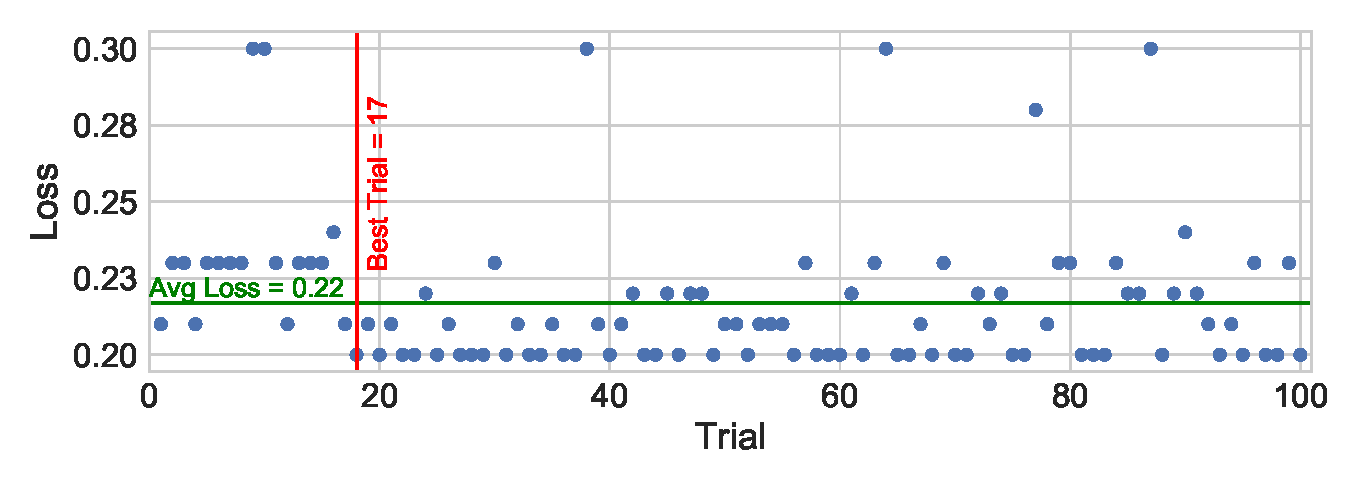
\includegraphics[width=\columnwidth]{../images/experiment-results/warm-starting-warm500-trials100-task31.eps}
        \caption{With Warmstarting}
    \end{subfigure}
    	\begin{subfigure}{\columnwidth}
        \centering
        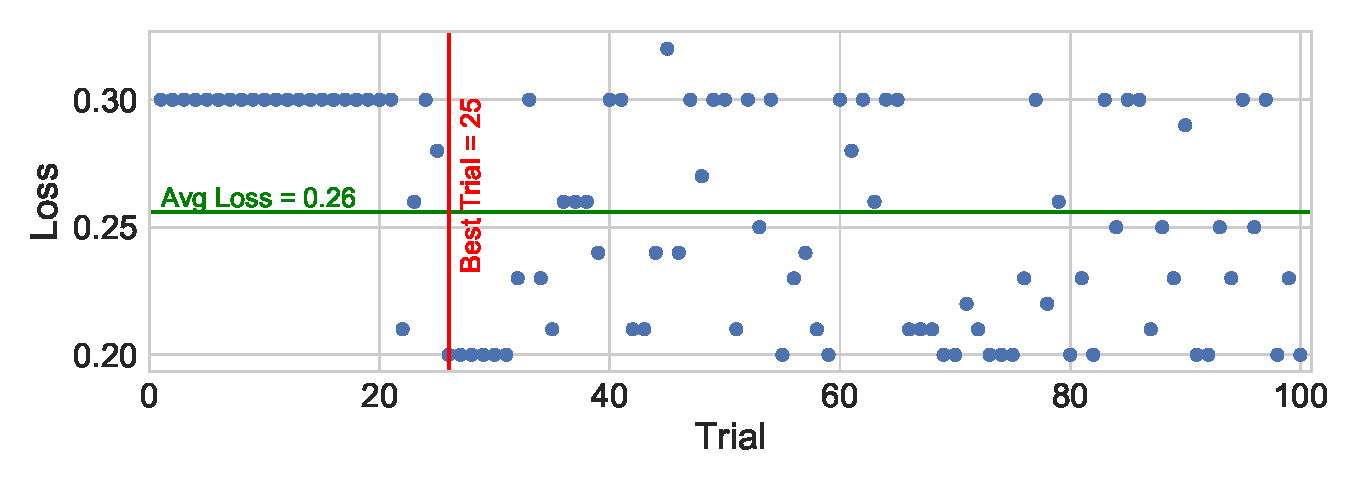
\includegraphics[width=\columnwidth]{../images/experiment-results/cold-starting-trials100-task31.eps}
        \caption{Without Warmstarting}
        \label{fig-warm-vs-cold-task-31}
    \end{subfigure}

\caption{Execution of 100 trials of bayesian optimization}
\label{deployment-quality-figure}
\end{figure}

\subsection{Time}
